%% Figure from MATH 556 notes, section 46 (Lecture 20). ADDED (not from lecture).
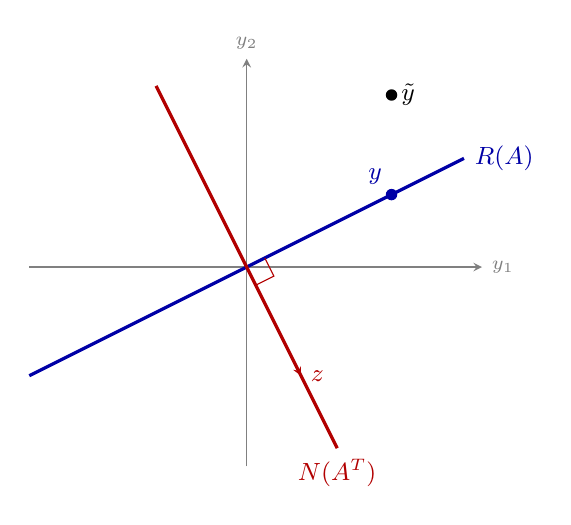
\begin{tikzpicture}[scale=1.15, >=stealth]
  \draw[->, gray] (-2.4,0) -- (2.6,0) node[right, font=\scriptsize] {$y_1$};
  \draw[->, gray] (0,-2.2) -- (0,2.3) node[above, font=\scriptsize] {$y_2$};
  \draw[very thick, blue!65!black] (-2.4,-1.2) -- (2.4,1.2) node[right, font=\small] {$R(A)$};
  \draw[very thick, red!70!black] (-1.0,2.0) -- (1.0,-2.0) node[below, font=\small] {$N(A^T)$};
  \draw[red!70!black] (0.2,0.1) -- (0.3,-0.1) -- (0.1,-0.2);
  \fill[blue!65!black] (1.6,0.8) circle (1.8pt) node[above left, font=\small] {$y$};
  \fill[black] (1.6,1.9) circle (1.8pt) node[right, font=\small] {$\tilde y$};
  \draw[->, red!70!black] (0,0) -- (0.6,-1.2) node[right, font=\small] {$z$};
\end{tikzpicture}
